\documentclass{article}
\usepackage{xparse}
\usepackage{graphicx}
\usepackage{float}
\usepackage[T1]{fontenc}
\usepackage[dvipsnames]{xcolor}
\usepackage{listings}
\usepackage{alloy-style}

\title{SafeStreets}
\author{Marco Premi, Fabrizio Siciliano, Giuseppe Taddeo}
\pagestyle{headings}

\begin{document}
\maketitle

\tableofcontents

\newpage
\section{Introduction}
\subsection{Purpose}
\subsubsection{General Purpose}
    The purpose of this document is to correctly analyze all requirements, goals
    and actions needed in order to correctly develop SafeStreets.\\
    \\
    SafeStreets is a crowd-sourced application that intends to provide users
    with the possibility to notify authorities when traffic violations occur
    (eg. traffic violations) and will help to maintain stability and order
    within the streets. A reporting system will also be available to police
    offices and municipality employees in order to allow them to analyze (and
    take actions accordingly) different areas of the city and assess which areas
    have the most violations committed in.\\
    \\
    The core application will focus on storing useful traffic violation data
    provided by users, mainly with the help of input forms and hard evidence
    such as images. At any violation input, SafeStreets will also store useful
    metadata such as date and time the violation was retrieved, geolocate where
    it is and update a city wide map highlighting the areas where violations
    happen.\\
    \\
    In addition to that, with the help of third parties (eg. municipality),
    SafeStreets will be able to retrieve the data given by such party and
    cross-reference them with its own data retrieved by users. By doing so, it
    will be possible to identify unsafe areas, assess which kind of problems
    happen more frequently and suggest possible intervention. It will also be
    possible for third parties (municipality and police officers) to
    automatically generate traffic tickets. This will be happening in order to
    cross-reference all available data in order to build statistics such as the
    most (or less) egregious offenders or the effectiveness of the SafeStreets
    initiative \subsubsection{Goals} Follows a list of all goals that will be
    reached with the SafeStreets initiative.
    \begin{itemize}
        \item $\langle$\textbf{G0}$\rangle$ The system will allow new customers
        to automatically sign up and create new accounts with the minimum
        required ID, email and password (all three will have to be valid);
        \item $\langle$\textbf{G1}$\rangle$ The systen will allow customers to
        sign in, upon check of the validity of email and password the customer
        inputs;
        \item $\langle$\textbf{G2}$\rangle$ The system will allow new traffic
        violations to be input by users, upon providing a list of required
        information;
        \item $\langle$\textbf{G3}$\rangle$ The system will provide an efficient
        reporting system in order to highlight different unsafe areas and will
        allow to filter the shown areas around the municipality; 
        \item $\langle$\textbf{G4}$\rangle$ The system will allow all customers
        to modify all account information and to delete the existing account; 
        \item $\langle$\textbf{G5}$\rangle$ The system will allow third parties
        to check all violations' details input in the municipality area, connect
        with an external software for photo forensics purposes and report the
        validity of the traffic violation in order to emit tickets or discard
        the violation itself.
    \end{itemize}
\subsection{Scope}
With SafeStreets users can notify the authorities when traffic violations occur,
and in particular parking violations. Both user and authorities must register to
the application and agree that SafeStreets stores the information provided,
completing it with suitable meta-data. The whole system, because it tracks users
information, must respect the standards defined for processing of sensitive
information such as GDPR if it is used in Europe. The user sends the type of the
violation to the municipality and direct proofs of it (like a photograph). The
system runs an algorithm to read the license plate and also asks the user to
directly insert the license for a better recognition. Of course other
information are required, like the name of the street when the violation has
occurred, which can be retrieved from user's direct input or from the
geographical position of the violation (using Google Maps API). Both users and
authorities can highlight the streets with the highest frequency of violations
or the vehicles that commit the most violations. SafeStreets crosses information
about the accidents that occur on the territory of the municipality with his own
data to identify potentially unsafe areas and suggest possible interventions.
Because municipality could generates traffic tickets from the information about
violations SafeStreets should guarantee that information is never altered (if a
manipulations occurs, the application should discard the information). Such
features are made possible trough the use of two mobile applications(one for the
citizens and one for the officers on the field). The collected information are
sent to a back-end. All the services can also be accessed through a specific
web-site. 
\subsection{Definitions, Acronyms, Abbreviations}
\subsubsection{Definitions}
\paragraph{User:} it is identified as a civilian customer of the product. It
will be the main source for the SafeStreets initiative to obtain information
about traffic violations and therefore be successful; \paragraph{Third
parties:}those kind of organization/company that could provide services useful
to SafeStreets and that will be able to retrieve data in order to improve the
streets' safety; \paragraph{Customer:} it defines both third party SafeStreets
users (police officers or municipality employees) and civilians;
\paragraph{Ghiro:} image manipulation detection software, used by third party
users in order to detect any image manipulation and assess the veracity of the
hard evidence connected to the traffic ticket
\subsubsection{Acronym}
\paragraph{UI:} User Interface \paragraph{GDPR:} General Data Protection
Regulation \paragraph{API:} Application Programming Interface \paragraph{GPS:}
Global Positioning System \paragraph{PO:} Police Officer \paragraph{ME:}
Municipality Employee
\subsubsection{Abbreviations}
\paragraph{Gn:} nth goal; \paragraph{Dn:} nth assumption; \paragraph{Rn:} nth
requirement; \paragraph{ID: } identifier (Fiscal Code fomunir Users, a
municipality identifier for Third Parties)
\subsection{Revision History}
\subsection{Reference Documents}
\begin{itemize}
    \item Specification document: "Mandatory Project Assignement AY 2019-2010"
    \item Alloy doc: http://alloy.lcs.mit.edu/alloy/documentation/quickguide/seq.html
    \item UML diagrams: https://www.uml-diagrams.org/
    \item Plate Recognizer: https://app.platerecognizer.com
    \item Ghiro: https://www.getghiro.org/
\end{itemize}
\subsection{Document Structure}
\paragraph{Chapter 1 - Introduction}
Gives an introduction to the problem by describing the purpose of SafeStreets.
It also shows the goals and the scope of the application. \paragraph{Chapter 2 -
Overall Description}Offers an overall description of the project. It identifies
the actors involved in the application and lists all the assumptions in order to
identify all the boundaries of the project. The product perspective includes
details on the shared phenomena and the domain models. The class diagram
describe the domain model used and the state diagrama analyzes:
\begin{itemize}
    \item The process of collecting violations from users
    \item The process of sharing informations with the municipality
\end{itemize}
The majority of functions of the system are more precisely specified by taking
in mind the goals of the system.  
\paragraph{Chapter 3 - Specific Requirements}
Contains external interface requirements which are: user interfaces, hardware
interfaces, software interfaces and communication interfaces. Few scenarios
describing how the system acts in real world are listed here. Furthermore it
provides the description of the functional requirements, through the use of use
cases and sequence diagrams. The non-functional requirements are defined through
performance requirements, design constraints and software system attributes.
\paragraph{Chapter 4 - Formal analysis using Alloy}
Includes the alloy model of some critical aspects with comments and
documentation.
\paragraph{Chapter 5 - Effort Spent}
Shows the effort spent by each single group member while working on the RASD.
\paragraph{Chapter 6 - References}
Includes the documents we used as reference.

\newpage
\section{Overall Description}
\subsection{Product Perspective}
afeStreets is designed to be a completely new software applications. It uses
some already proven services (like Google Maps and PlateRecognizer APIs) for its
critical tasks. The software uses these services in order to double check
whether both addresses and license plates are correctly standardized in order to
be stored into the violations database.\\
The system is composed of two different mobile applications: one for the
citizens that want to reports violations and one for the officers acting on the
field. It also provides a web site for third party users which allows them to
assess and analyze potential unsafe areas, thanks also to a powerful reporting
system.\\
Taken into consideration that the municipality could generate traffic tickets
from the input violations, the software will be critical when it comes to
handling chain of custody. The latter is assured to never be broken by not
allowing any kind of customer (user, PO or employee) to modify the reported
violation. Supposedly, when some traffic violations might be erroneous or do not
have any reason of existence, the inputting user can warn the responsible third
party by attaching a warning explaining why it should not be taken into
consideration. The systems also ensures the veracity of each violation and the
hard evidence attached to it by running a image manipulation detection software
(Ghiro, per instance). This process is used by third parties before the emission
of each ticket to the corresponding offender.\\
\\
A high-level class diagram can be found below, which provides a model of the
application domain. The most important classes (not all of those which will be
implemented once the software will be ready) are shown in order to define how
the different components of SafeStreets will be communicating with each other.
It is possible to identify two kinds of third party users: police officers and
municipality employees. The first ones will be given access to both mobile
application and web application; the latter will be provided access just to the
above mentioned web application which will help these users assess the veracity
of the hard evidence attached to the traffic violations and to further analyze
unsafe areas around the municipality.\\

\begin{figure}[H]
    \centering
    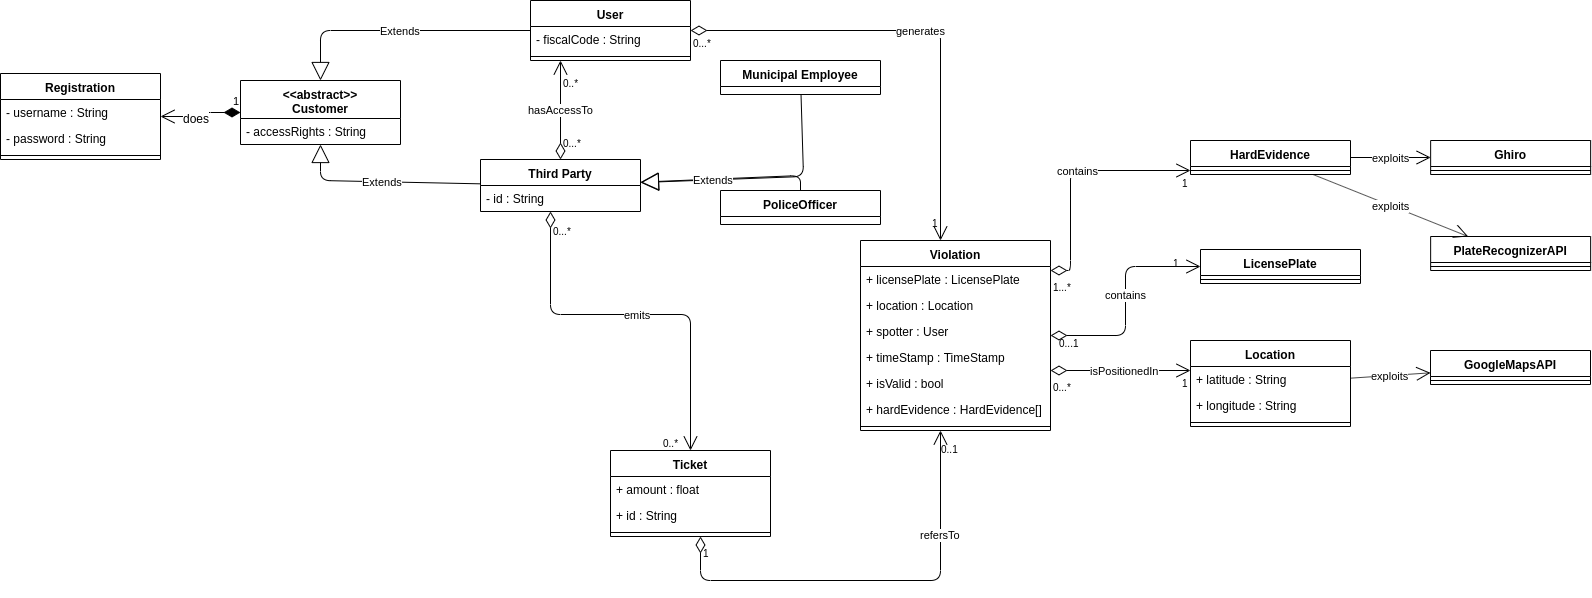
\includegraphics[scale=0.255]{Images/umlmodel}
    \caption{Class diagram}
\end{figure}

It is possible to notice that there are two actors that model the third party.
Police Officers and municipality employees have both access to a web version of
the application, since this version provides the tools for checking input
violations, emit traffic tickets and assess possible improvements to unsafe
areas.\\
\\
We will now furtherly analize some critical aspects of the system with the use
of activity diagrams. Actual system functions will not be presented, just some
high level system main processes.

\begin{figure}[H]
    \centering
    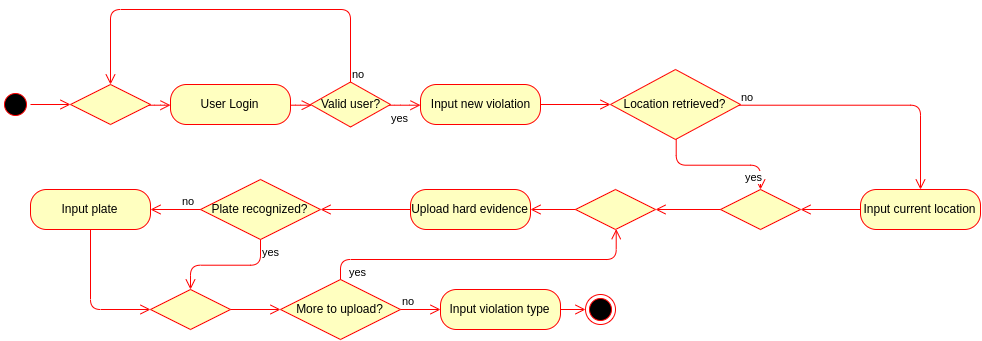
\includegraphics[scale=0.36]{Images/ActivityInputViolation}
    \caption{Activity Diagram: Input violation}
\end{figure}

It is easily understandable that for any unathorized user trying to access the
system (those who have not correctly signed up) is not possible to input any new
violation. Furthermore, the location retrieving and the plate recognizing
processes are a bit tricky. The system tries to execute both of them
automatically by calling the respective API from GoogleMaps or PlateRecognizer.
If one (or both) processes fail, the system recognizes the problem and asks the
user to input the missing piece of information. Once all information is ready,
everything is sent to a shared database and saved for future check by third
party employees (PO or ME). 


\begin{figure}[H]
    \centering
    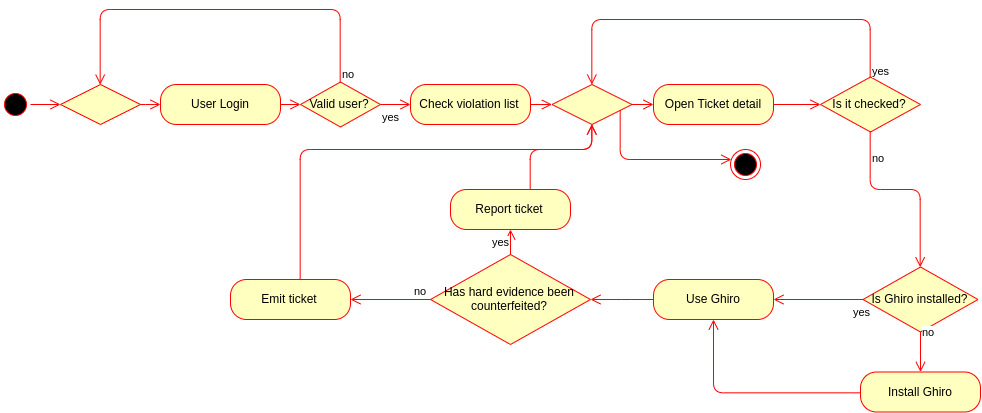
\includegraphics[scale=0.36]{Images/ActivityCheckViolation}
    \caption{Activity Diagram: Checking violation}
\end{figure}

As it is mentioned by the description above this one, no user can access the
system without a proper username and password. What is interesting in this part
of the process, is the possibility to end the whole process only once the
traffic violation has been checked, which means that the hard evidence attached
to it has to be approved as not being counterfeited or else. A running version
of the Ghiro software has to be already installed on the machine which is
accessing the system through a web browser; if not, the system itself will
automatically redirect to the latest downloadable version of it. 

\subsection{Product Functions}
In the following section the most important product functions of the system are
reported.
    \subsubsection{Reporting traffic violations}
    This function is the main action that the user can use. After having logged
    in within its application, pressing on "Report Infraction" the system will
    ask to insert an image specifying its format and characteristics (clear
    image, defined context, visible plate). Once the image is loaded, the system
    will ask him to enter the type of infraction reported, the date and time, as
    well as the position detected by GPS signal or manually via user input. At
    this point the user will confirm the data entered and save the report.
    Moreover he will see in his personal area, under the list of his reports,
    the new report with all the data he has entered. In addition, the report
    will be added to the list of reports made in the same municipality.

    \subsubsection{Police Officer - Reportings Management (APP)}
    This function allows the police officer to have in real time all the reports
    made in his municipality of competence. In fact, after logging into his
    application and providing his identification as a police officer, the
    application through an analysis system of the latter will identify the
    municipality of competence of the agent and will show him the list of all
    the appropriate reports. He can therefore go to the place of the report to
    resolve the infraction manually by clicking "Resolve Live" and closing the
    infraction or, in the event that the violation can no longer be assessed in
    person (i.e. the car has moved) he can leave the report opened to then
    resolve it from the website.

    \subsubsection{Police Officer - Reportings Management (WEB)}
    This function allows the police officer to resolve the reports (i.e.
    generating a traffic ticket for the owner of the machine) via the website
    without being physically present on the spot. Once logged in using codes
    provided by the municipality, the police officer will be able to see all the
    reports still open (i.e. no one has clicked "Resolve Live") and analyze
    them. He can take the photo posted by the user and submit it to specialized
    programs to ensure that it is not tampered with and will therefore be able
    to generate the ticket and close the report.

    \subsubsection{Municipal Employee - Interventions Management}
    This function allows a municipal employee, after logging in through his own
    identifier, to be able to view all the reports made in the municipality of
    competence and be able to insert in the application the accident data that
    occur in the territory. In this way, by pressing the "Start Analysis"
    button, SafeStreets will identify potentially unsafe areas and show them to
    the municipal employee and the municipal employee will be able to decide
    whether to take precautions (i.e. insert barrier between cycle path and
    road).

\subsection{User characteristics}
The actors of the application are the following:
\begin{itemize}
    \item User: a customer of the service who, after having installed the
    application on his mobile device, having registered through univocal
    identification data and accepted the processing of his data and the civil
    and criminal liability of his own reports, can post an infraction report
    attaching a photo of this (with clear and legible license plate) followed by
    date, time and position (the latter acquired by GPS detection or manual
    entry)
    \item Authority: a customer who uses the system based on its role;
    \begin{itemize}
        \item Policeman: after installing the application on his mobile device,
        having registered through univocal data and codes provided by your
        municipality, he have the possibility to see the list of reports of
        infractions made in the Municipality of his competence and also has the
        ability to access to the system through a website to carry out analysis
        of the reports (image photoshop) and generate traffic ticket to the
        accused.
        \item Municipal Employee: through the website, he has access to the
        unsafe areas of his own Municipality to decide road interventions to be
        applied within it
        \item Municipal Director: through the website, he has access to both
        reports and traffic tickets both to unsafe areas and to statistical data
        produced by SafeStreets in order to assess the effectiveness of the
        application.
    \end{itemize}
\end{itemize}
\subsection{Assumptions, dependencies and constraints}
\subsubsection{Assumptions}
\begin{itemize}
    \item $\langle$\textbf{D0}$\rangle$ The device acquires users' location with
    an error of 5 meters at most.
    \item $\langle$\textbf{D1}$\rangle$ Each fiscal code is unique.
    \item $\langle$\textbf{D2}$\rangle$ Each authorithies ID is unique.
    \item $\langle$\textbf{D5}$\rangle$ The system automatically recognizes the
    city using the Authorities ID.
    \item $\langle$\textbf{D3}$\rangle$ Once a violation has been saved it can't
    be modified.
    \item $\langle$\textbf{D4}$\rangle$ The system is always able to contact to
    user in order to ask him/her more information.
    \item $\langle$\textbf{D5}$\rangle$ If the customer is connected to internet
    he/she is always able to contact the system.
\end{itemize}
\subsubsection{Dependencies}
The system uses external suitable services to make its architecture simpler.
\begin{itemize}
    \item PlateRecognizer API
    \item Google Maps API
    \item Ghiro
\end{itemize}
\subsubsection{Constraints}
\paragraph{2.4.3.1 Regulatory policies}\mbox{}\\
SafeStreets uses sensitive data which handling differs from nation to nation.
For example, in UE, GDPR provides the guidelines to transmit, store and analyze
information.\\ SafeStreets personalizes the process according to the country in
which the services are used. \paragraph{2.4.3.2 Parallel Operations}\mbox{}\\
The system must provide support for multiple parallel operations from a big
number of different users. The user must not wait in order to be able to connect
to the service.
\newpage
\section{Specific Requirements}
\subsection{External Interface Requirements}
\subsubsection{User Interfaces}
\begin{figure}[H]
    \centering
    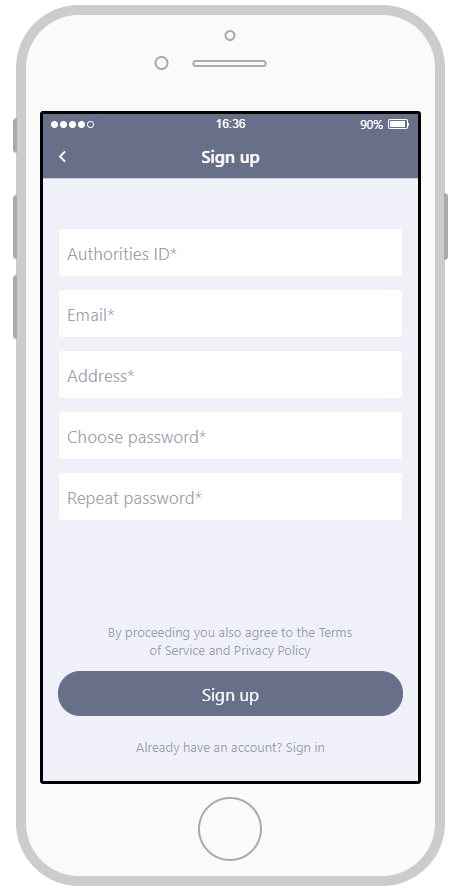
\includegraphics[scale=0.7]{Images/SignUpAuthoritiesApp}
    \caption{SignUp authorities}
\end{figure}
\begin{figure}[H]
    \centering
    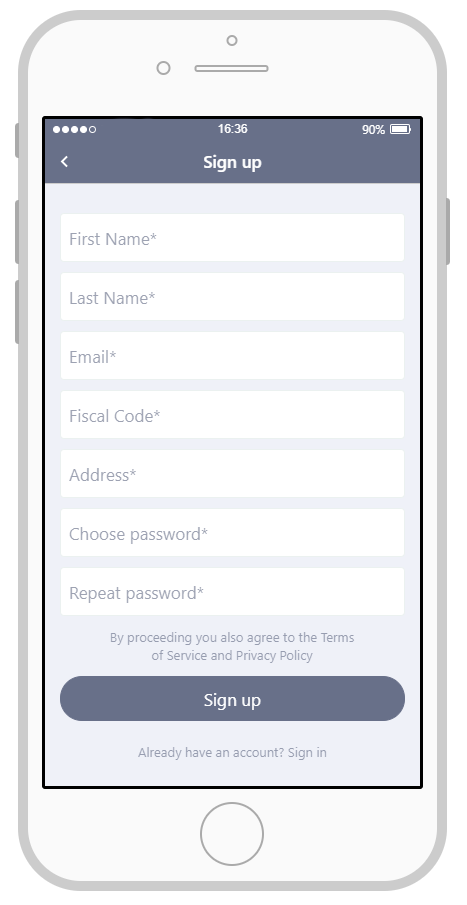
\includegraphics[scale=0.7]{Images/SignUpUtenteAPP}
    \caption{SignUp User}
\end{figure}
\begin{figure}[H]
    \centering
    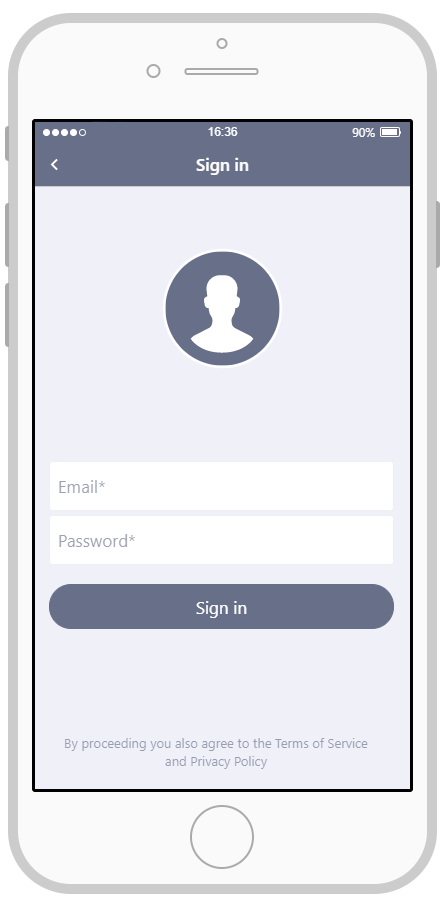
\includegraphics[scale=0.7]{Images/SignInAPP}
    \caption{SignIn}
\end{figure}
\begin{figure}[H]
    \centering
    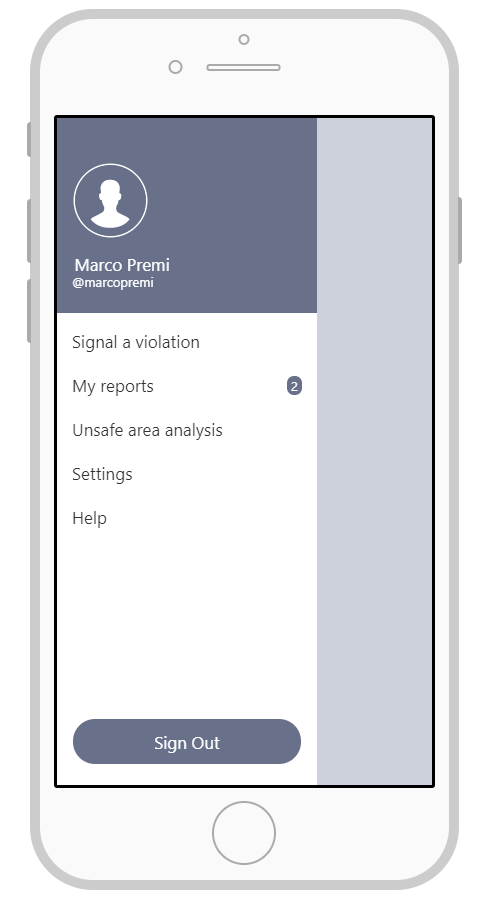
\includegraphics[scale=0.7]{Images/MenuAPP}
    \caption{Menu}
\end{figure}
\begin{figure}[H]
    \centering
    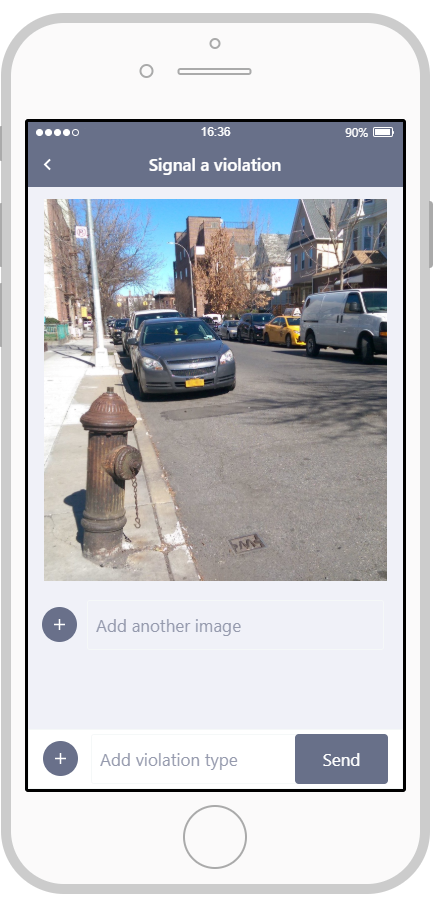
\includegraphics[scale=0.7]{Images/SignalAViolationAPP}
    \caption{SignIn}
\end{figure}
\begin{figure}[H]
    \centering
    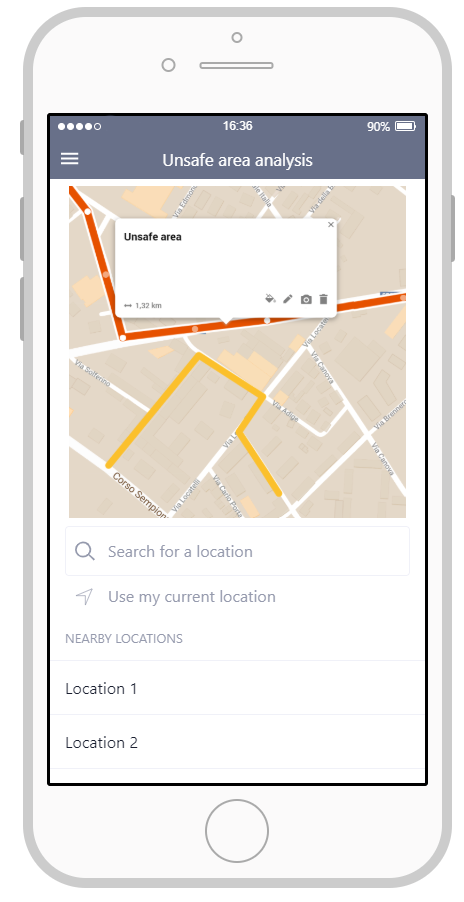
\includegraphics[scale=0.7]{Images/UnsafeAreaAnalysisAPP}
    \caption{SignIn}
\end{figure}
\begin{figure}[H]
    \centering
    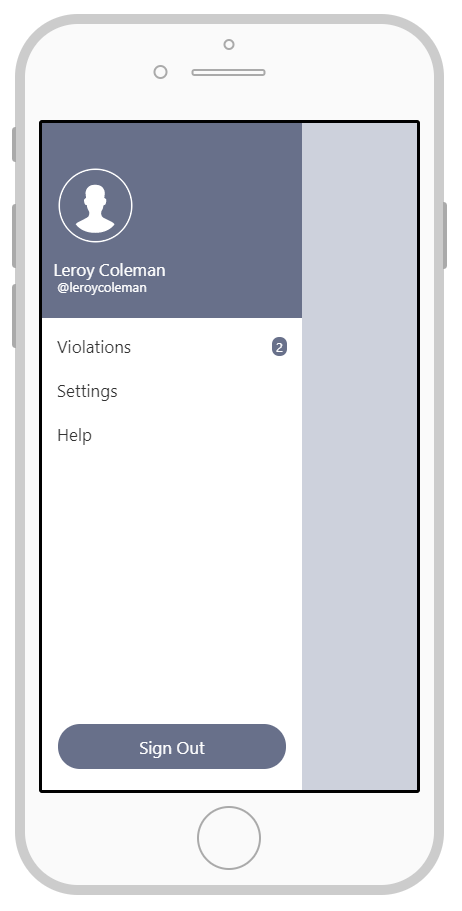
\includegraphics[scale=0.7]{Images/MenuOfficerAPP}
    \caption{Officer Menu}
\end{figure}
\begin{figure}[H]
    \centering
    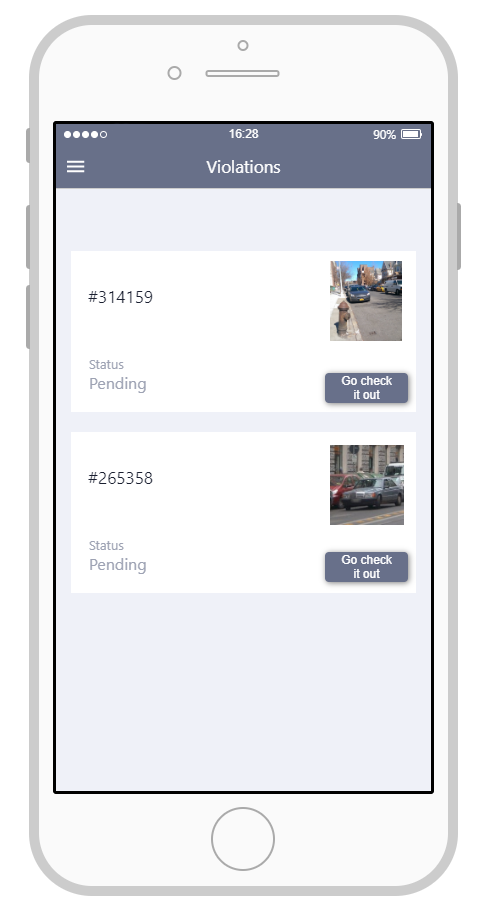
\includegraphics[scale=0.7]{Images/ViolationsAPP}
    \caption{Violations check}
\end{figure}
\begin{figure}[H]
    \centering
    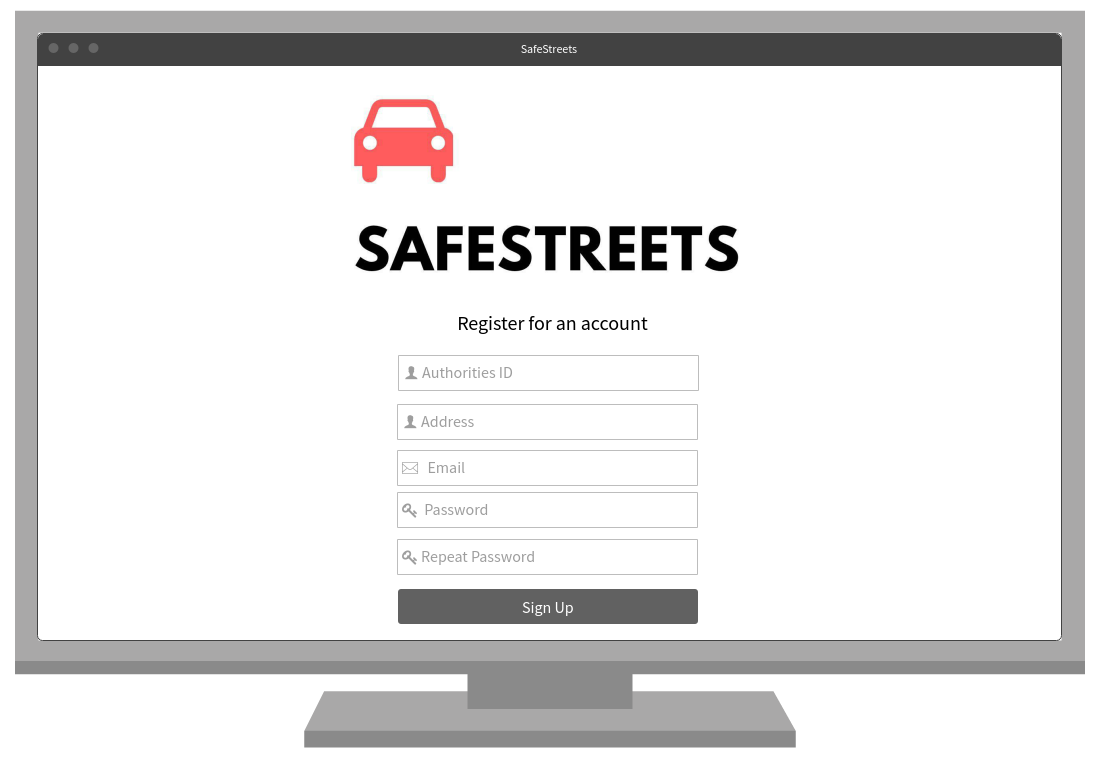
\includegraphics[scale=0.35]{Images/WEBSignUp}
    \caption{SignUp}
\end{figure}
\begin{figure}[H]
    \centering
    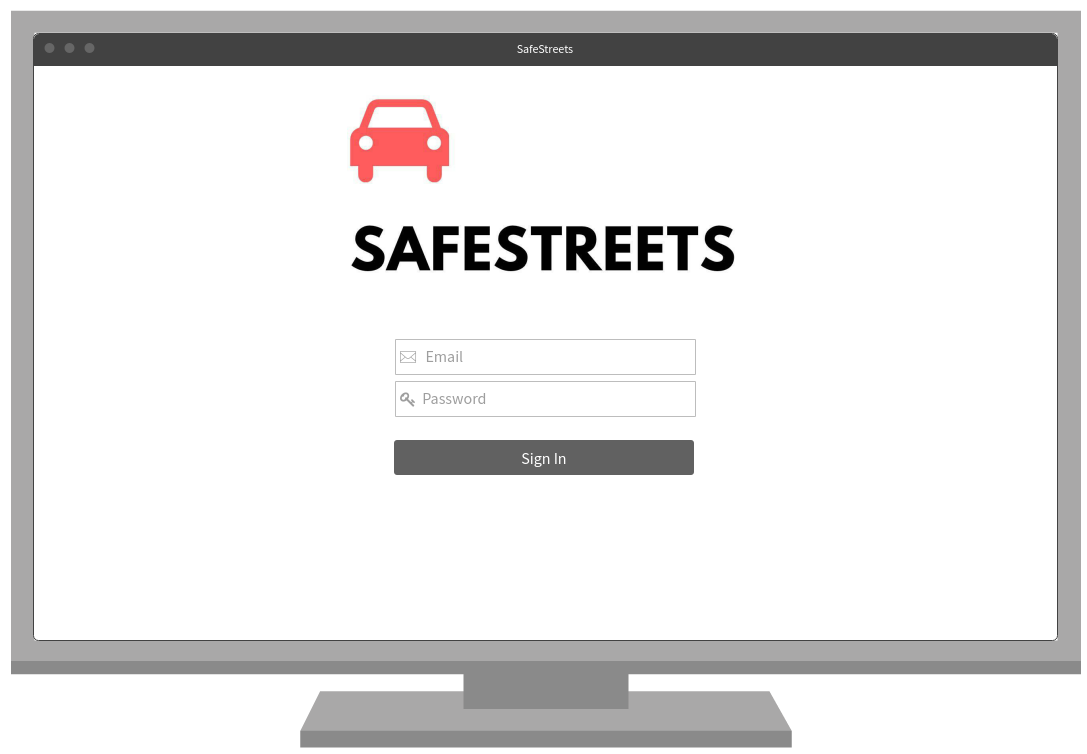
\includegraphics[scale=0.35]{Images/WEBSignIn}
    \caption{SignIn}
\end{figure}
\begin{figure}[H]
    \centering
    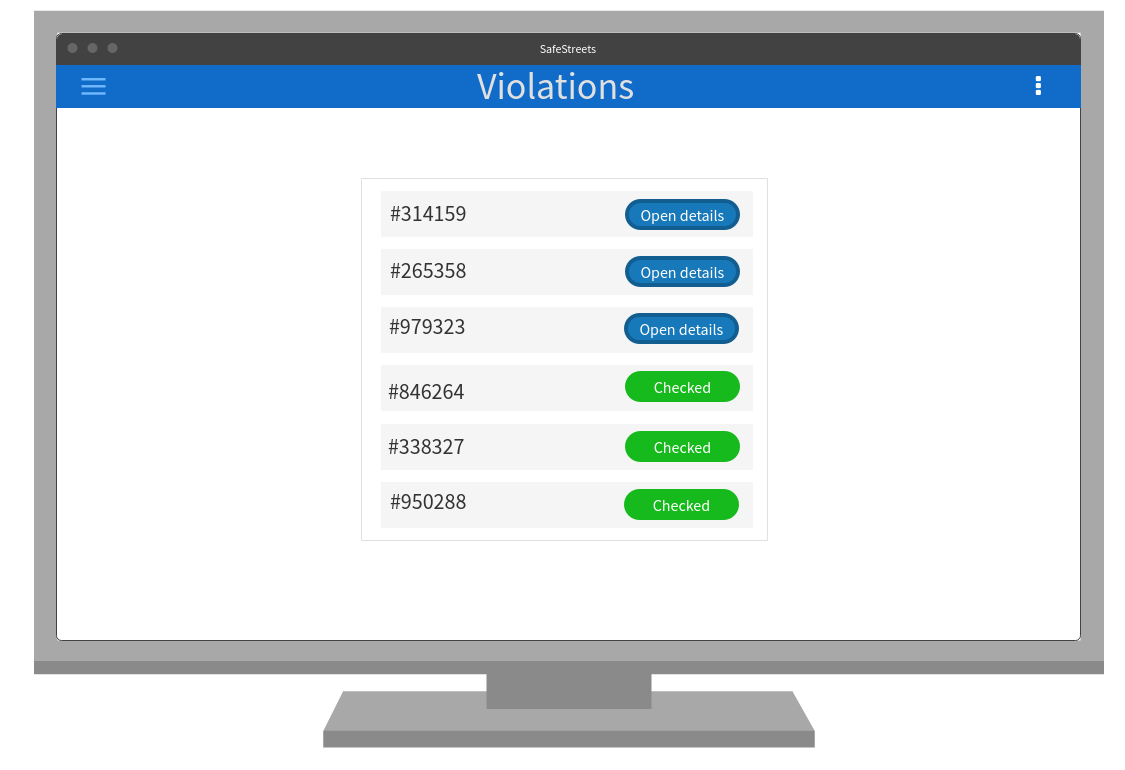
\includegraphics[scale=0.35]{Images/WEBViolations}
    \caption{Violations}
\end{figure}
\begin{figure}[H]
    \centering
    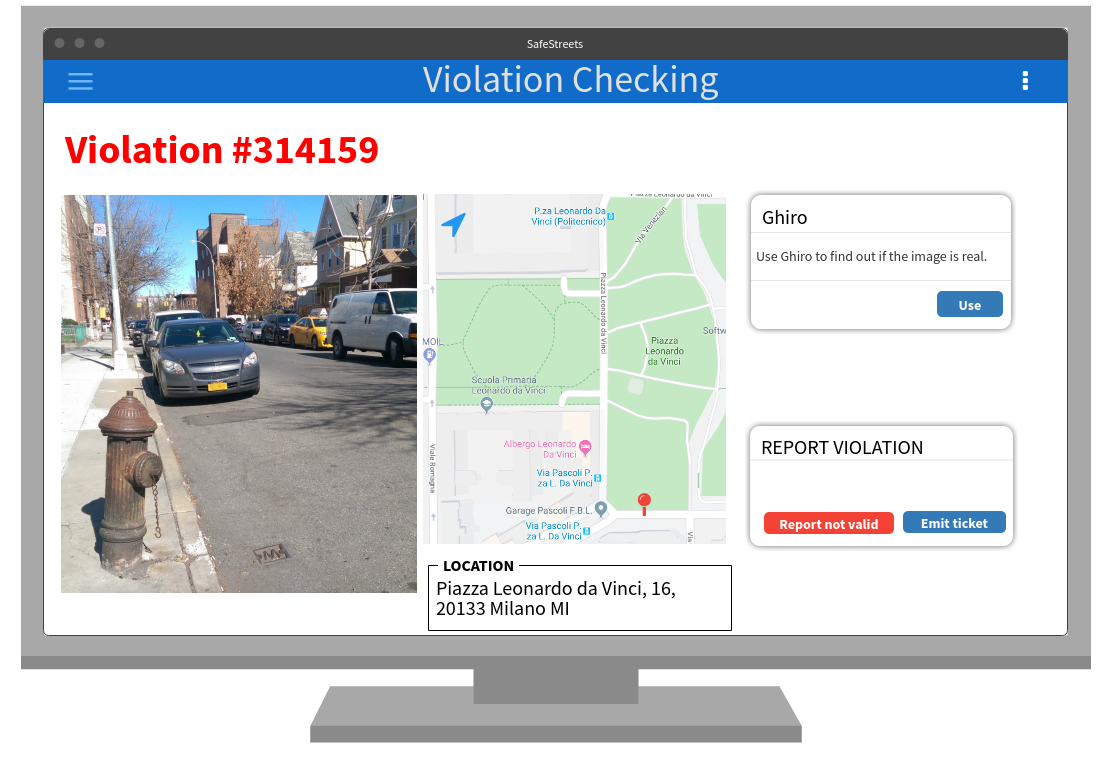
\includegraphics[scale=0.35]{Images/WEBViolationChecking}
    \caption{Violations checking}
\end{figure}
\begin{figure}[H]
    \centering
    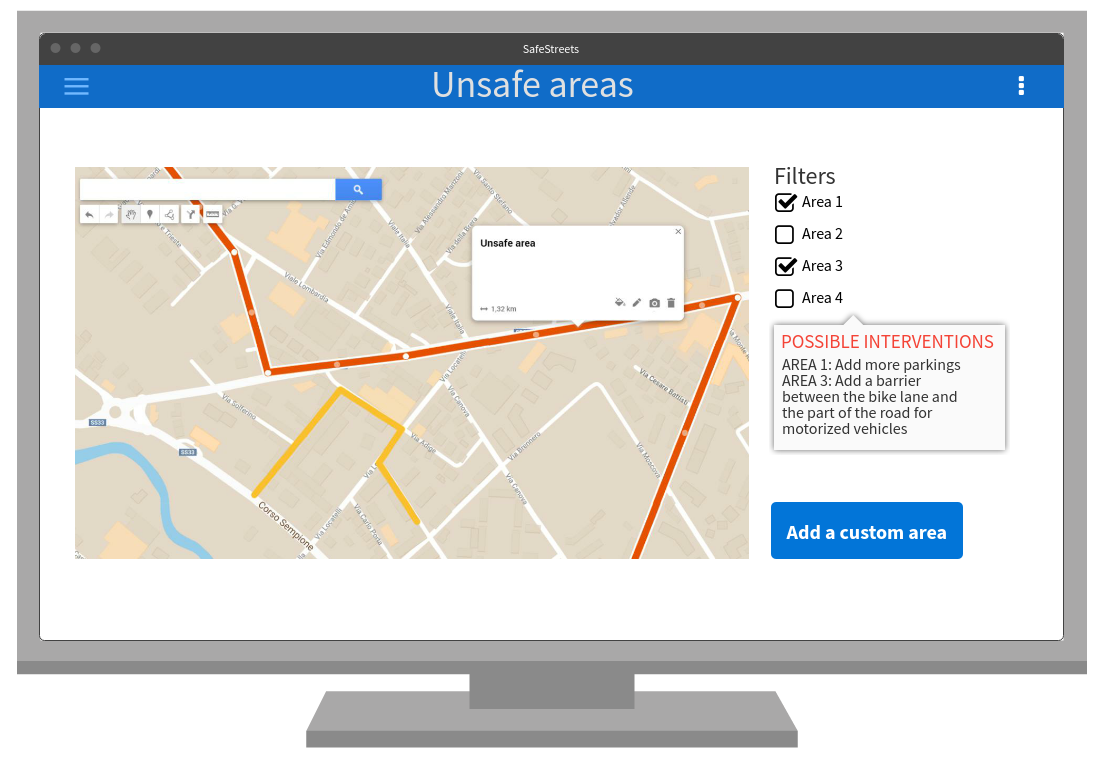
\includegraphics[scale=0.35]{Images/WEBUnsafeAreas}
    \caption{Unsafe Areas}
\end{figure}
\newpage
\newpage
\subsubsection{Hardware Interfaces}
The system has no hardware interfaces.
\subsubsection{Software Interfaces}
The system doesn't provide any API to external applications.\\
However some softwares part of SafeStreets is developed by other companies.
\begin{itemize}
    \item Google Maps API: for localization and creation of unsafe areas.
    \item Plate Recognizer API: for License Plate recognition.
    \item Ghiro: a digital image forensics tool used for find out if the image
    in the violation report is real.
\end{itemize}
\subsubsection{Communication Interfaces}
The system only uses HTTP(more precisely HTTPS) as communication service.
HTTP/HTTPS is used for:
\begin{itemize}
    \item User and third parties registration.
    \item Sending violations both to SafeStreets and to authorities.
    \item Using Google Maps API and Plate Recognizer API
\end{itemize}
\subsection{Scenarios}
\subsection{Functional requirements}
\paragraph{User}\mbox{}\\
$\langle$\textbf{G0}$\rangle$ SignUp to the system
\begin{description}
    \item $\langle$\textbf{R1}$\rangle$ the customer must not be already
    registered  in the system
    \item $\langle$\textbf{R2}$\rangle$ the customer must provide a valid ID and
    email
    \item $\langle$\textbf{R3}$\rangle$ the customer must agree to the Terms of
Use \end{description}\mbox{}\\
$\langle$\textbf{G1}$\rangle$ SignIn to the system
\begin{description}
    \item $\langle$\textbf{R4}$\rangle$ the customer must be already sign up
    \item $\langle$\textbf{R5}$\rangle$ the customer must insert its email and
    password \end{description}\mbox{}\\\\
$\langle$\textbf{G2}$\rangle$ Signal a violation
\begin{description}
    \item $\langle$\textbf{R6}$\rangle$ the user must be able to insert one or
    more photos of the violation
    \item $\langle$\textbf{R7}$\rangle$ the user must send information about its
    location
    \item $\langle$\textbf{R8}$\rangle$ the user can add the type of violation
    that is being reported
\end{description}
$\langle$\textbf{G3}$\rangle$ Show Unsafe Areas
\begin{description}
    \item $\langle$\textbf{R9}$\rangle$ the user is shown the unsafe areas
    around him
    \item $\langle$\textbf{R10}$\rangle$ the customer is allowed to filter the
    unsafe areas
    \item $\langle$\textbf{R11}$\rangle$ the customer is allowed to search
    unsafe areas 
\end{description}    
$\langle$\textbf{G4}$\rangle$ Manage Account
\begin{description}
    \item $\langle$\textbf{R12}$\rangle$ the customer must be able to modify its
    account information
    \item $\langle$\textbf{R13}$\rangle$ the customer must be able to delete
    his/her account
\end{description}

\paragraph{Sequence diagrams}

\begin{figure}[H]
    \centering
    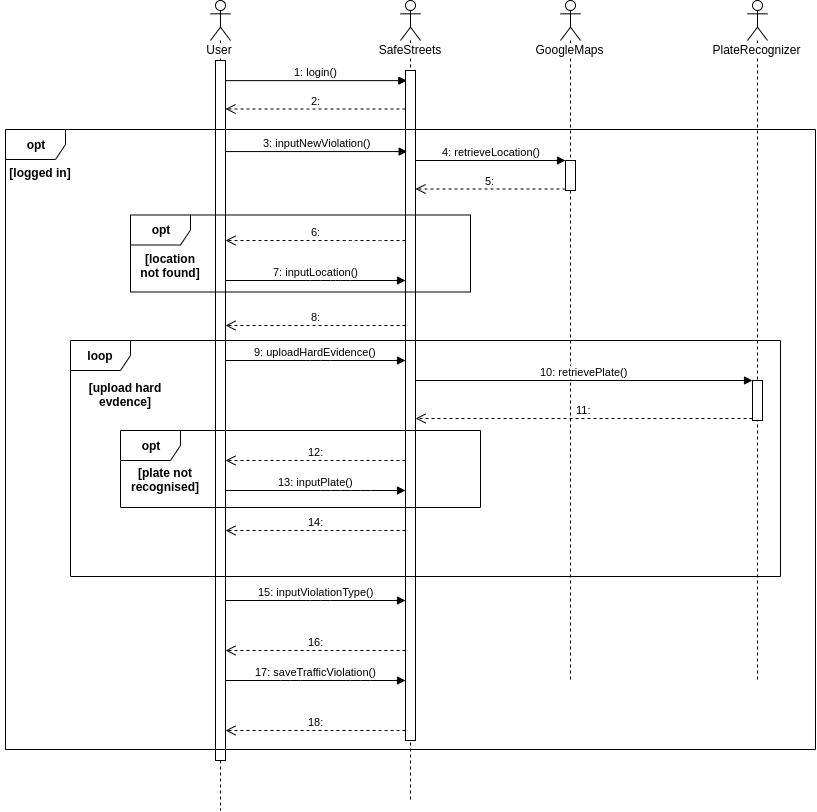
\includegraphics[scale=0.45]{Images/SequenceReportViolation}
    \caption{Sequence diagram: input traffic violation}
\end{figure}

\begin{figure}[H]
    \centering
    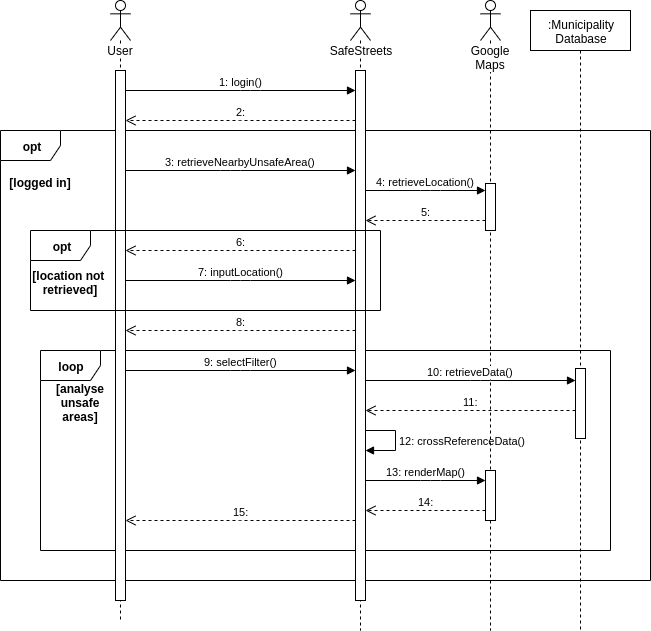
\includegraphics[scale=0.5]{Images/SequenceUserAnalyseUnsafeAreas} 
    \caption{Sequence diagram: analyse unsafe areas}
\end{figure}

\paragraph{Third parties}\mbox{}\\
$\langle$\textbf{G0}$\rangle$ SignUp to the system
\begin{description}
    \item $\langle$\textbf{R1}$\rangle$ the customer must not be already
    registered  in the system
    \item $\langle$\textbf{R2}$\rangle$ the customer must provide a valid ID and
    email
    \item $\langle$\textbf{R3}$\rangle$ the customer must agree to the Terms of
Use \end{description}\mbox{}\\
$\langle$\textbf{G1}$\rangle$ SignIn to the system
\begin{description}
    \item $\langle$\textbf{R4}$\rangle$ the customer must be already signed up
    \item $\langle$\textbf{R5}$\rangle$ the customer must insert its email and
    password\\
\end{description}
$\langle$\textbf{G5}$\rangle$ Check Violations
\begin{description}
    \item $\langle$\textbf{R14}$\rangle$ the third party must be able to check
    all the new and past violations details
    \item $\langle$\textbf{R15}$\rangle$ the third party must be able to use
    Ghiro
    \item $\langle$\textbf{R16}$\rangle$ the third party must be able to report
    the validity of the violation \end{description}\mbox{}\\
$\langle$\textbf{G3}$\rangle$ Show Unsafe Areas
\begin{description}
    \item $\langle$\textbf{R10}$\rangle$ the customer is allowed to filter the
    unsafe areas
    \item $\langle$\textbf{R11}$\rangle$ the customer is allowed to search
    unsafe areas 
    \item $\langle$\textbf{R17}$\rangle$ the third party is shown a list of
    possible improvements to be made to the shown areas by the system
\end{description}
$\langle$\textbf{G4}$\rangle$ Manage Account
\begin{description}
    \item $\langle$\textbf{R12}$\rangle$ the customer must be able to modify its
    account information
    \item $\langle$\textbf{R13}$\rangle$ the customer must be able to delete
    his/her account
\end{description}    

\begin{figure}[H]
    \centering
    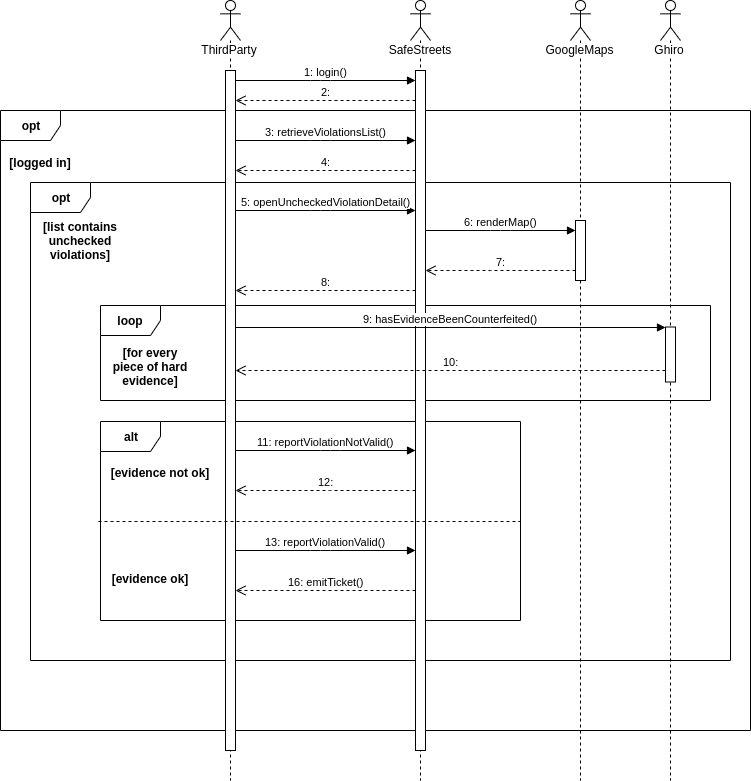
\includegraphics[scale=0.47]{Images/SequenceThirdPartyCheckViolation} 
    \caption{Sequence diagram: check violation and report its validity}
\end{figure}

\begin{figure}[H]
    \centering
    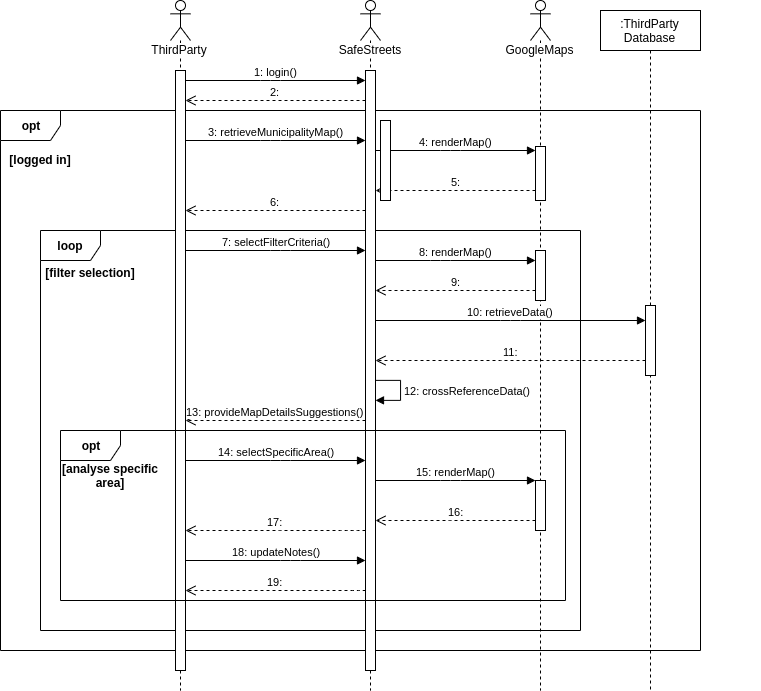
\includegraphics[scale=0.47]{Images/SequenceThirdPartyUnsafeAreas} 
    \caption{Sequence diagram: analyse unsafe areas}
\end{figure}


\subsection{Use Cases}
\subsubsection{User use cases}
\begin{figure}[H]
    \centering
    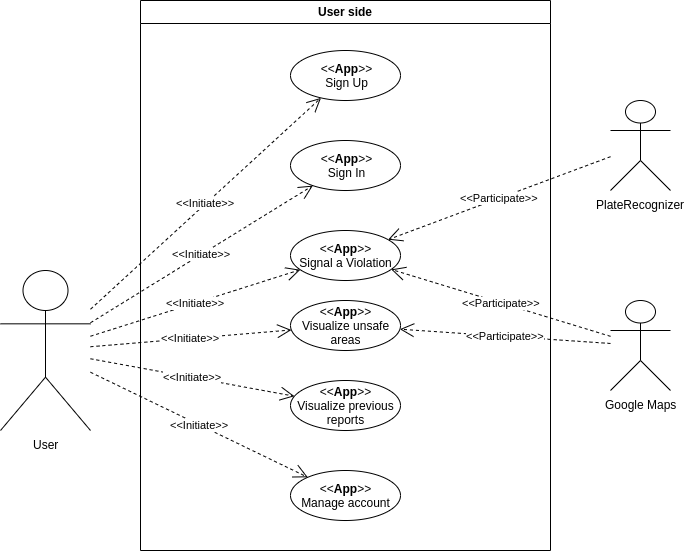
\includegraphics[scale=0.5]{Images/UseCaseUserView}
    \caption{Use Case Diagram: User}
\end{figure}

\begin{table}[H]
    \begin{tabular}{|l|l|}
    \hline
    Name & \textbf{Sign Up} \\ \hline  
    Actor & User\\ \hline 
    Entry conditions &  The user has downloaded the application on his/her
    device\\ \hline 
    Events flow & 
    \begin{minipage}[t]{0.7\textwidth}
    \begin{enumerate}
        \item The user opens the application on his/her device
        \item The user clicks on "Sign Up" button
        \item The user fills the registration form with all the mandatory fields
        \item The user clicks the confirmation button
        \item The system saves the data
    \end{enumerate}
    \end{minipage} \\ \hline
    Exit conditions & \begin{minipage}[t]{0.7\textwidth}The system has stored
    user data, the user is registered and now is able to use te application
    \end{minipage}\\ \hline
    Exceptions & \begin{minipage}[t]{0.7\textwidth} \begin{enumerate}
        \item The user was already signed up
        \item The user doesn't fill all the mandatory fields with valid data
        \item The email or the fiscal code is already registered
        \item The user closes the application before the process has ended
    \end{enumerate}\end{minipage} \\ \hline
    \end{tabular}
\end{table}

\begin{table}[H]
    \begin{tabular}{|l|l|}
    \hline
    Name &\begin{minipage}[t]{0.7\textwidth} \textbf{Sign In} \end{minipage} \\
    \hline  
    Actor & \begin{minipage}[t]{0.7\textwidth} User \end{minipage} \\ \hline 
    Entry conditions & \begin{minipage}[t]{0.7\textwidth} \begin{enumerate}
        \item The user has already downloaded the the application on his/her
        device
        \item The user has already signed up
    \end{enumerate}
    \end{minipage} \\ \hline 
    Events flow & \begin{minipage}[t]{0.7\textwidth}
    \begin{enumerate}
        \item The user opens the application on his/her device
        \item The user inserts his/her credentials in the "Email" and "Password"
        fields.
        \item The user clicks on the "Sign In" button
    \end{enumerate}
    \end{minipage} \\ \hline
    Exit conditions & \begin{minipage}[t]{0.7\textwidth} The user is
    successfully signed in \end{minipage} \\ \hline
    Exceptions & \begin{minipage}[t]{0.7\textwidth}
    \begin{enumerate}
        \item The user inserts invalid Email
        \item The user inserts invalid Password   
        \item The user closes the application before the process has ended 
    \end{enumerate}
    \end{minipage} \\ \hline
    \end{tabular}
\end{table}

\begin{table}[H]
    \begin{tabular}{|l|l|}
    \hline
    Name & \begin{minipage}[t]{0.7\textwidth} \textbf{Signal a
    violation}\end{minipage} \\ \hline  
    Actor & \begin{minipage}[t]{0.7\textwidth} User\end{minipage} \\ \hline 
    Entry conditions & \begin{minipage}[t]{0.7\textwidth} The user has already
    logged in \end{minipage} \\ \hline 
    Events flow & \begin{minipage}[t]{0.7\textwidth}
    \begin{enumerate}
        \item The user opens the Menu
        \item The user clicks on "Signal a violation" button in the Menu
        \item The user uploads one or more photos
        \item The user adds additional information
        \item The user adds one or more violation types
        \item The user clicks "Send"
        \item SafeStreets receives the violation
    \end{enumerate}
    \end{minipage} \\ \hline
    Exit conditions & \begin{minipage}[t]{0.7\textwidth}The user has
    successfully reported a violation \end{minipage} \\ \hline
    Exceptions & \begin{minipage}[t]{0.7\textwidth}
    \begin{enumerate}
        \item The user closes the application before the process has ended 
        \item The user doesn't have internet connection 
    \end{enumerate}    
    \end{minipage} \\ \hline
    \end{tabular}
\end{table}


\begin{table}[H]
    \begin{tabular}{|l|l|}
    \hline
    Name & \begin{minipage}[t]{0.7\textwidth} \textbf{Visualize unsafe areas}
    \end{minipage} \\ \hline  
    Actor & \begin{minipage}[t]{0.7\textwidth} User \end{minipage} \\ \hline 
    Entry conditions & \begin{minipage}[t]{0.7\textwidth} The user has already
    logged in\end{minipage} \\
    \hline 
    Events flow & \begin{minipage}[t]{0.7\textwidth} 
    \begin{enumerate}
        \item The user opens the Menu
        \item The user clicks on the "Unsafe area analysis" button in the Menu
        \item The user is allowed to select different filters and the area
        he/she wants to see
    \end{enumerate}
    \end{minipage} \\ \hline
    Exit conditions & \begin{minipage}[t]{0.7\textwidth} The user can see all
    the unsafe areas proposed by SafeStreets and the third party\end{minipage}
    \\
    \hline
    Exceptions & \begin{minipage}[t]{0.7\textwidth}  The user doesn't have
    internet connection \end{minipage} \\ \hline
    \end{tabular}
\end{table}

\begin{table}[H]
    \begin{tabular}{|l|l|}
    \hline
    Name & \begin{minipage}[t]{0.7\textwidth} \textbf{Visualize previous
    reports}\end{minipage} \\ \hline  
    Actor & \begin{minipage}[t]{0.7\textwidth} User\end{minipage} \\ \hline 
    Entry conditions & \begin{minipage}[t]{0.7\textwidth} The user has already
    logged in \end{minipage} \\
    \hline 
    Events flow & \begin{minipage}[t]{0.7\textwidth} 
    \begin{enumerate}
        \item The user opens the Menu
        \item The user selects the "My reports" button in the Menu
        \item The user is allowed to see all the previous reports he/she made
    \end{enumerate}    
    \end{minipage} \\ \hline
    Exit conditions & \begin{minipage}[t]{0.7\textwidth} The user is provided
    with the requested data \end{minipage} \\
    \hline
    Exceptions & \begin{minipage}[t]{0.7\textwidth} The user doesn't have
    internet connection  \end{minipage} \\ \hline
    \end{tabular}
\end{table}

\begin{table}[H]
    \begin{tabular}{|l|l|}
    \hline
    Name & \begin{minipage}[t]{0.7\textwidth} \textbf{Manage Account}
    \end{minipage} \\ \hline  
     Actor & \begin{minipage}[t]{0.7\textwidth} User \end{minipage} \\ \hline 
     Entry conditions & \begin{minipage}[t]{0.7\textwidth} The user has already
     logged in \end{minipage} \\
     \hline 
     Events flow & \begin{minipage}[t]{0.7\textwidth} 
    \begin{enumerate}
        \item The user opens the Menu
        \item The user selects the "Settings" button in the Menu
        \item The user is allowed to change his/her adress, the password, the
        email or to delete the account
    \end{enumerate}    
    \end{minipage} \\ \hline
     Exit conditions & \begin{minipage}[t]{0.7\textwidth} New user settings are
     saved to his/her account or the account is deleted \end{minipage} \\
     \hline
     Exceptions & \begin{minipage}[t]{0.7\textwidth} The user closes the
     application before the process has ended \end{minipage} \\ \hline
    \end{tabular}
\end{table}

\subsubsection{Third party use cases}

\begin{figure}[H]
    \centering
    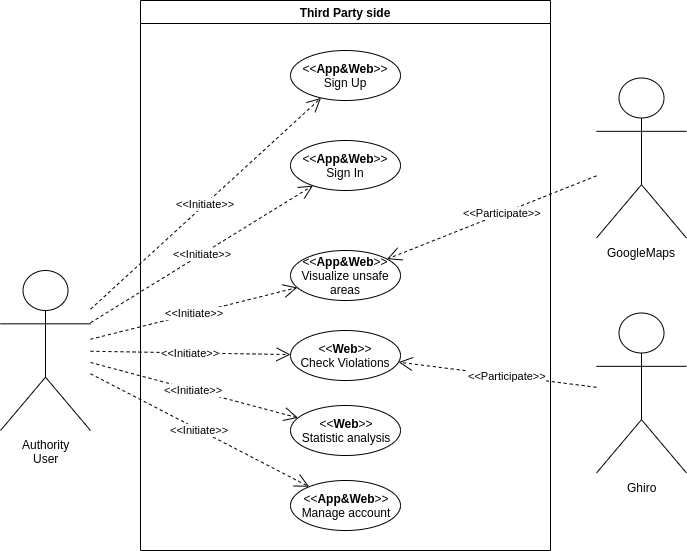
\includegraphics[scale=0.5]{Images/UseCaseThirdPartyView}
    \caption{Use Case Diagram: Third Party}
\end{figure}

\begin{table}[H]
    \begin{tabular}{|l|l|}
    \hline
     Name & \begin{minipage}[t]{0.7\textwidth}\textbf{Sign Up}\end{minipage} \\
     \hline  
     Actor & \begin{minipage}[t]{0.7\textwidth} Third party\end{minipage} \\
     \hline 
     Entry conditions & \begin{minipage}[t]{0.7\textwidth} The third party is
     not already registered\end{minipage} \\
     \hline 
     Events flow & \begin{minipage}[t]{0.7\textwidth} 
    \begin{enumerate}
        \item The third party accesses SafeStreets website
        \item The third party is asked to sign in
        \item The third party clicks on "Sign Up"
        \item The third party fills the registration form with all the mandatory
        fields
        \item The third party clicks the confirmation button
        \item The system saves the data
    \end{enumerate}
    \end{minipage} \\ \hline
     Exit conditions & \begin{minipage}[t]{0.7\textwidth} The system has stored
     third party data, the third party is registered and now is able to use the
     website\end{minipage} \\
     \hline
     Exceptions & \begin{minipage}[t]{0.7\textwidth}
    \begin{enumerate}
        \item The third party was already signed up
        \item The third party doesn't fill all the mandatory fields with valid
        data
        \item The email or the AuthoritiesID is already registered
        \item The third party closed the application beforse the process has
        ended
    \end{enumerate}    
    \end{minipage} \\ \hline
    \end{tabular}
\end{table}

\begin{table}[H]
    \begin{tabular}{|l|l|}
    \hline
    Name & \begin{minipage}[t]{0.7\textwidth}\textbf{Sign In} \end{minipage} \\
    \hline  
    Actor & \begin{minipage}[t]{0.7\textwidth} Third party \end{minipage} \\
    \hline 
    Entry conditions & \begin{minipage}[t]{0.7\textwidth} The third party has
    already signed up\end{minipage} \\
    \hline 
    Events flow & \begin{minipage}[t]{0.7\textwidth}
    \begin{enumerate}
        \item The third party accesses SafeStreets website
        \item The third party is asked to sign in
        \item The third party inserts the credentials in the "Email" and
        "Password" fields.
        \item The third party clicks on "Sign In"
    \end{enumerate}    
    \end{minipage} \\ \hline
    Exit conditions & \begin{minipage}[t]{0.7\textwidth} The third party is
    successfully signed in \end{minipage} \\
    \hline
    Exceptions & \begin{minipage}[t]{0.7\textwidth}
    \begin{enumerate}
        \item The third party inserts invalid Email
        \item The third party inserts invalid Password
        \item The third party closes the website before the process has ended
    \end{enumerate}
    \end{minipage} \\ \hline
    \end{tabular}
\end{table}

\begin{table}[H]
    \begin{tabular}{|l|l|}
    \hline
    Name & \begin{minipage}[t]{0.7\textwidth}\textbf{Unsafe Areas}
    \end{minipage} \\ \hline  
    Actor & \begin{minipage}[t]{0.7\textwidth} Third party \end{minipage} \\
    \hline 
    Entry conditions & \begin{minipage}[t]{0.7\textwidth} The third party has
    already logged in\end{minipage} \\
    \hline 
    Events flow & \begin{minipage}[t]{0.7\textwidth}
    \begin{enumerate}
        \item The third party clicks on the menu icon
        \item The third party click on "Unsafe ares"
        \item The third party is allowed create and delete unsafe areas, to
        select different filters and to search different areas
    \end{enumerate} 
    \end{minipage} \\ \hline
    Exit conditions & \begin{minipage}[t]{0.7\textwidth} The unsafe areas editor
    is presented to the third party\end{minipage} \\
    \hline
    Exceptions & \begin{minipage}[t]{0.7\textwidth} \end{minipage} \\ \hline
    \end{tabular}
\end{table}

\begin{table}[H]
    \begin{tabular}{|l|l|}
    \hline
    Name & \begin{minipage}[t]{0.7\textwidth}\textbf{Check Violations}
    \end{minipage} \\ \hline  
    Actor & \begin{minipage}[t]{0.7\textwidth} Third party \end{minipage} \\
    \hline 
    Entry conditions & \begin{minipage}[t]{0.7\textwidth} The third party has
    already logged in \end{minipage} \\
    \hline 
    Events flow & \begin{minipage}[t]{0.7\textwidth}
    \begin{enumerate}
        \item The third party clicks on the menu icon
        \item The third party clicks on "Violations"
        \item The third party is allowed to see the list of previous and actual
        violations (checked or not)
        \item The third party click on "Open Details" of one particular not
        checked violation
        \item The third party is allowed to see information about the particular
        violation
        \item The third party can click "Use" on Ghiro card to find out if the
        image is real
        \item The third party can click "Report not valid" if the image is fake
        or "Report valid" if the image is real
    \end{enumerate}
    \end{minipage} \\ \hline
    Exit conditions & \begin{minipage}[t]{0.7\textwidth} The third party can
    manage the violations \end{minipage} \\
    \hline
    Exceptions & \begin{minipage}[t]{0.7\textwidth}The third party closes the
    website before the process has ended \end{minipage} \\ \hline
    \end{tabular}
\end{table}

\begin{table}[H]
    \begin{tabular}{|l|l|}
    \hline
    Name & \begin{minipage}[t]{0.7\textwidth}\textbf{Manage Account}
    \end{minipage} \\ \hline  
    Actor & \begin{minipage}[t]{0.7\textwidth}Third party\end{minipage} \\
    \hline 
    Entry conditions & \begin{minipage}[t]{0.7\textwidth} The third party has
    already logged in \end{minipage} \\
    \hline 
    Events flow & \begin{minipage}[t]{0.7\textwidth}
    \begin{enumerate}
        \item The third party clicks on the menu icon
        \item The third party click on "Manage Account"
        \item The third party is allowed to change the email, the password or to
        delete the account
    \end{enumerate}
    \end{minipage} \\ \hline
    Exit conditions & \begin{minipage}[t]{0.7\textwidth} New user settings are
    saved to the third party account or the account is deleted\end{minipage} \\
    \hline
    Exceptions & \begin{minipage}[t]{0.7\textwidth}The third party closes the
    website before the process has ended \end{minipage} \\ \hline
    \end{tabular}
\end{table}

\begin{table}[H]
    \begin{tabular}{|l|l|}
    \hline
    Name & \begin{minipage}[t]{0.7\textwidth}\textbf{Check violations on the
    field} \end{minipage} \\ \hline  
    Actor & \begin{minipage}[t]{0.7\textwidth} Third party(officer)
    \end{minipage} \\ \hline 
    Entry conditions & \begin{minipage}[t]{0.7\textwidth}The third party has
    already logged in \end{minipage} \\
    \hline 
    Events flow & \begin{minipage}[t]{0.7\textwidth} 
    \begin{enumerate}
        \item The third party opens the Menu
        \item The third party clicks on "Violations" button in the Menu
        \item The third party is allowed to see the list of violations
        \item The third party clicks on "Go check it out" button
        \item SafeStreets opens Google Maps or one other turn-by-turn navigation
        app to reach the violation location
    \end{enumerate}
    \end{minipage} \\ \hline
    Exit conditions & \begin{minipage}[t]{0.7\textwidth} The officer can reach
    the violation location\end{minipage} \\
    \hline
    Exceptions & \begin{minipage}[t]{0.7\textwidth} 
    \begin{enumerate}
        \item The officer closes the application before the process has ended
        \item The officer doesn't have internet connection 
    \end{enumerate}    
    \end{minipage} \\ \hline
    \end{tabular}
\end{table}


\subsection{Performance requirements}
The system is provided to serve a great number of users and third parties
simultaneously. The back-end must be powerful enough to accept thousands of
requests at same time during all the day.\\
The front-end applications (mobile and web) don't have particular performance
requirements.
\subsection{Design Constraints}
\subsubsection{Standars compliance}
With regard to the privacy, security for the mobile application and the back-end
is a big issue, so the whole project is subject to the the GDPR. Furthermore
it's a good practice to apply W3C's Standards to ensure intercompatibility.
\subsubsection{Hardware Limitations}
Even if SafeStreets is a software-based service there are some hardware
limitations regarding the smartphones.
\begin{itemize}
    \item must be able to make HTTPS requests (connection to internet
    4G/3G/2G/Wi-Fi)
    \item must have on board GPS (mobile devices only)
\end{itemize}
\subsubsection{Any Other Constraint}
%probabilmente da cancellare (Secondo me non ci sono, a parere mio)
\subsection{Software System Attributes}
\subsubsection{Reliability}
The system must be able to run 24/7 without any interruptions. Only small
concessions from this requirement might be tolerated. The system must also be
fault tolerant. In order to exploit this last point the data saved on the
servers should be duplicated.
\subsubsection{Availability}
Maximum availability is a necessity because users should be able to report
violations 24/7. One or two days per year may be used for maintainance, so
availability of 99\% is expected.
\subsubsection{Security}
User and third party provide data that contains sensitive information, so the
security aspect is of primary relevance.\\ Communications between user, third
party and SafeStreets must be encrypted and the database with all the data must
be protected from any possibile internal or external attack.
\subsubsection{Mantainability}
The system shoule be flexibile and easy to mantain. For this purpose the whole
system will be developed using a modular architecture. \\
Fixing and modifying the system will be easy with the modular architecture.

\subsubsection{Portability}
SafeStreets in order to be useful must be used by a very large number of people.
It is for this reason that third parties' registration website must be available
on the majority of browsers (Firefox, Google Chrome, Safari, Opera, Microsoft
Edge and Internet Explorer 11).\\
Naturally the mobile application must be available on both Android and iOs.

\newpage
\section{Formal Analysis using Alloy}
\lstinputlisting[language=alloy,basicstyle=\normalsize]{RASD.als}

\newpage
\section{Effort spent}
\begin{center}
    \begin{tabular}{|c|c|c|c|c|}
        \hline
        \textbf{Description of the task} & \textbf{MP} & \textbf{FS} &
        \textbf{GT} \\
        \hline
        Introduction                    & 2.5   & 2     & 0     \\
        Overall Description             & 3     & 8     & 2     \\
        Specific requirements           & 0     & 4     & 0     \\
        Formal analysis using Alloy     & 0     & 0     & 10    \\
        \hline
    \end{tabular}
\end{center}

    
\end{document}  